\documentclass{standalone}
\usepackage[utf8]{inputenc}
\usepackage[T1]{fontenc}
\usepackage[turkish]{babel}
\usepackage{tikz}
\usetikzlibrary{arrows.meta,shapes}
\begin{document}
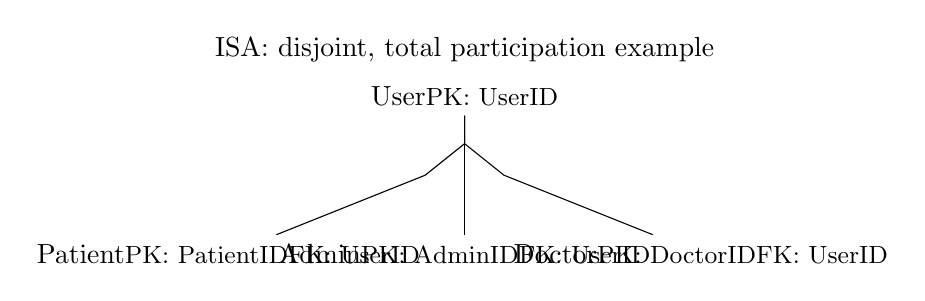
\begin{tikzpicture}
  \tikzset{entity/.style={draw, rectangle, minimum width=3.0cm, minimum height=0.8cm, align=center}}
  \node[entity] (User) at (0,0) {User\\{\small PK: UserID}};
  \node[entity] (Patient) at (-3,-2) {Patient\\{\small PK: PatientID\\FK: UserID}};
  \node[entity] (Doctor) at (3,-2) {Doctor\\{\small PK: DoctorID\\FK: UserID}};
  \node[entity] (Admin) at (0,-2) {Admin\\{\small PK: AdminID\\FK: UserID}};

  % ISA lines
  \draw (User) -- (0,-0.6) -- (-0.5,-1) -- (Patient);
  \draw (User) -- (0,-0.6) -- (0.5,-1) -- (Doctor);
  \draw (User) -- (0,-0.6) -- (0,-1) -- (Admin);

  \node at (0,0.6) {ISA: disjoint, total participation example};
\end{tikzpicture}
\end{document}
